%\placelogofalse
\section{Methodology}
\begin{frame}{Sourcing MKL Versions}
  \begin{outline}
    \1 Intel only releases from the last year on their software center.
    \1 Releases through 2023 through Intel's apt repository
    \1 Some 2020 releases on Archive.org
    \1 Official MKL python wheels on pypi include dynamic libraries as far back as 2018
    \2 All benchmarks used dynamic linking as fewer static libraries could not be sourced
  \end{outline}
\end{frame}

\begin{frame}{Experimental Setup}
\begin{columns}
\column{0.48\linewidth}
\textbf{Benchmarks}
\begin{outline}
  \1 One warm-up iteration
  \1 $16$ timed iterations
  \1 Plots show average time
  \1 Error bars show standard deviation
  \1 Sequential and OpenMP variants 
  \2 $80$ threads for OpenMP builds
  \2 2025.0 build of Intel's OpenMP runtime used for all benchmarks 
\end{outline}

\column{0.48\linewidth}
\textbf{Machine}
\begin{outline}
  \1 IceLake node on TACC 
  \1 Intel Xeon Platinum 8380 (Q2'21)
  \1 80 cores on two sockets 
\end{outline}
  Workloads sizes differ for most experiments between sequential and OpenMP builds
\end{columns}
\end{frame}

\placelogofalse
\begin{frame}{Overview  - All}
\begin{outline}
\1 All experiments (except pardiso - OpenMP)
\1 Performance normalized to 2018.0.3
\1 2025 average is $0.98$
\1 Median normalized performance as dashed line 
\end{outline}
\begin{center}
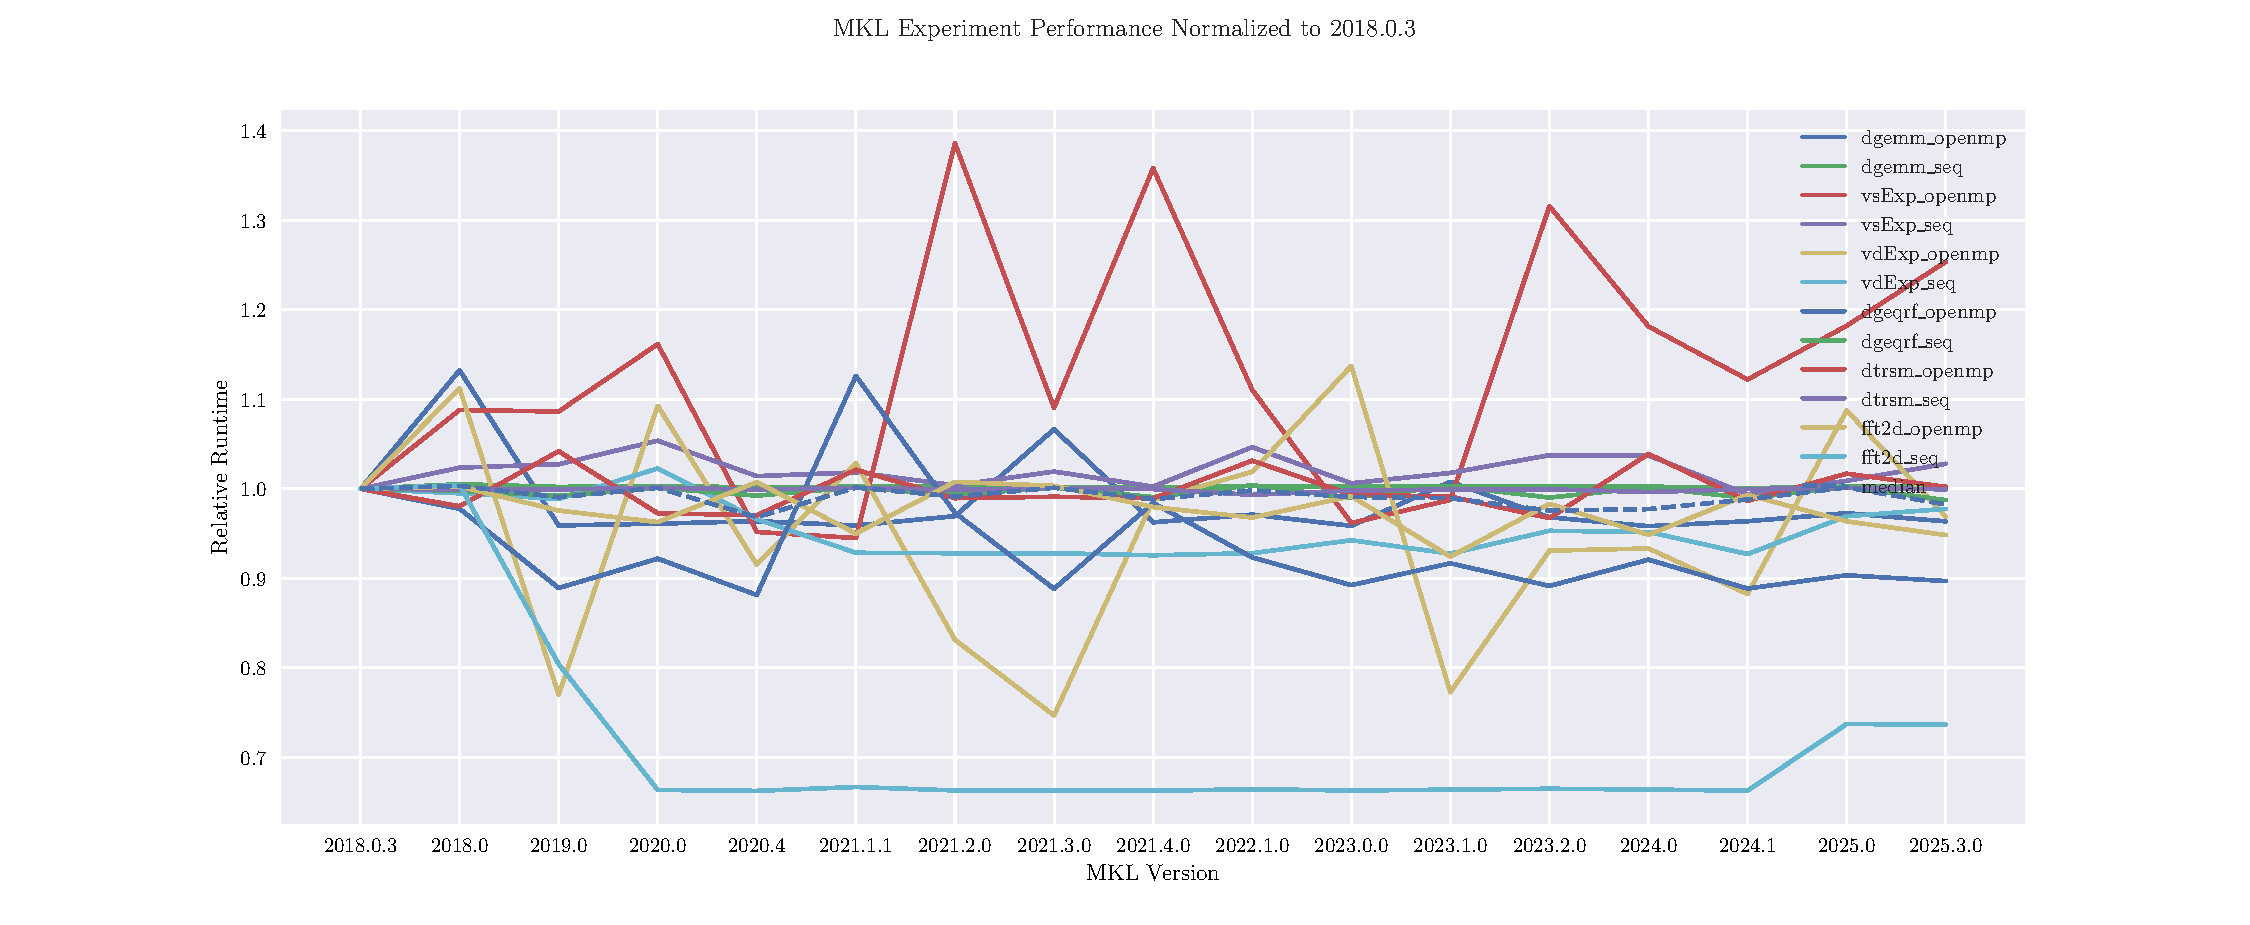
\includegraphics[width=12cm, page=1]{assets/overview.pdf}
\end{center}
\end{frame}

\placelogofalse
\begin{frame}{Overview  - Sequential}
\begin{outline}
\1 All sequential experiments 
\1 Performance normalized to 2018.0.3
\1 2025 average is $0.95$
\1 Median normalized performance as dashed line 
\end{outline}
\begin{center}
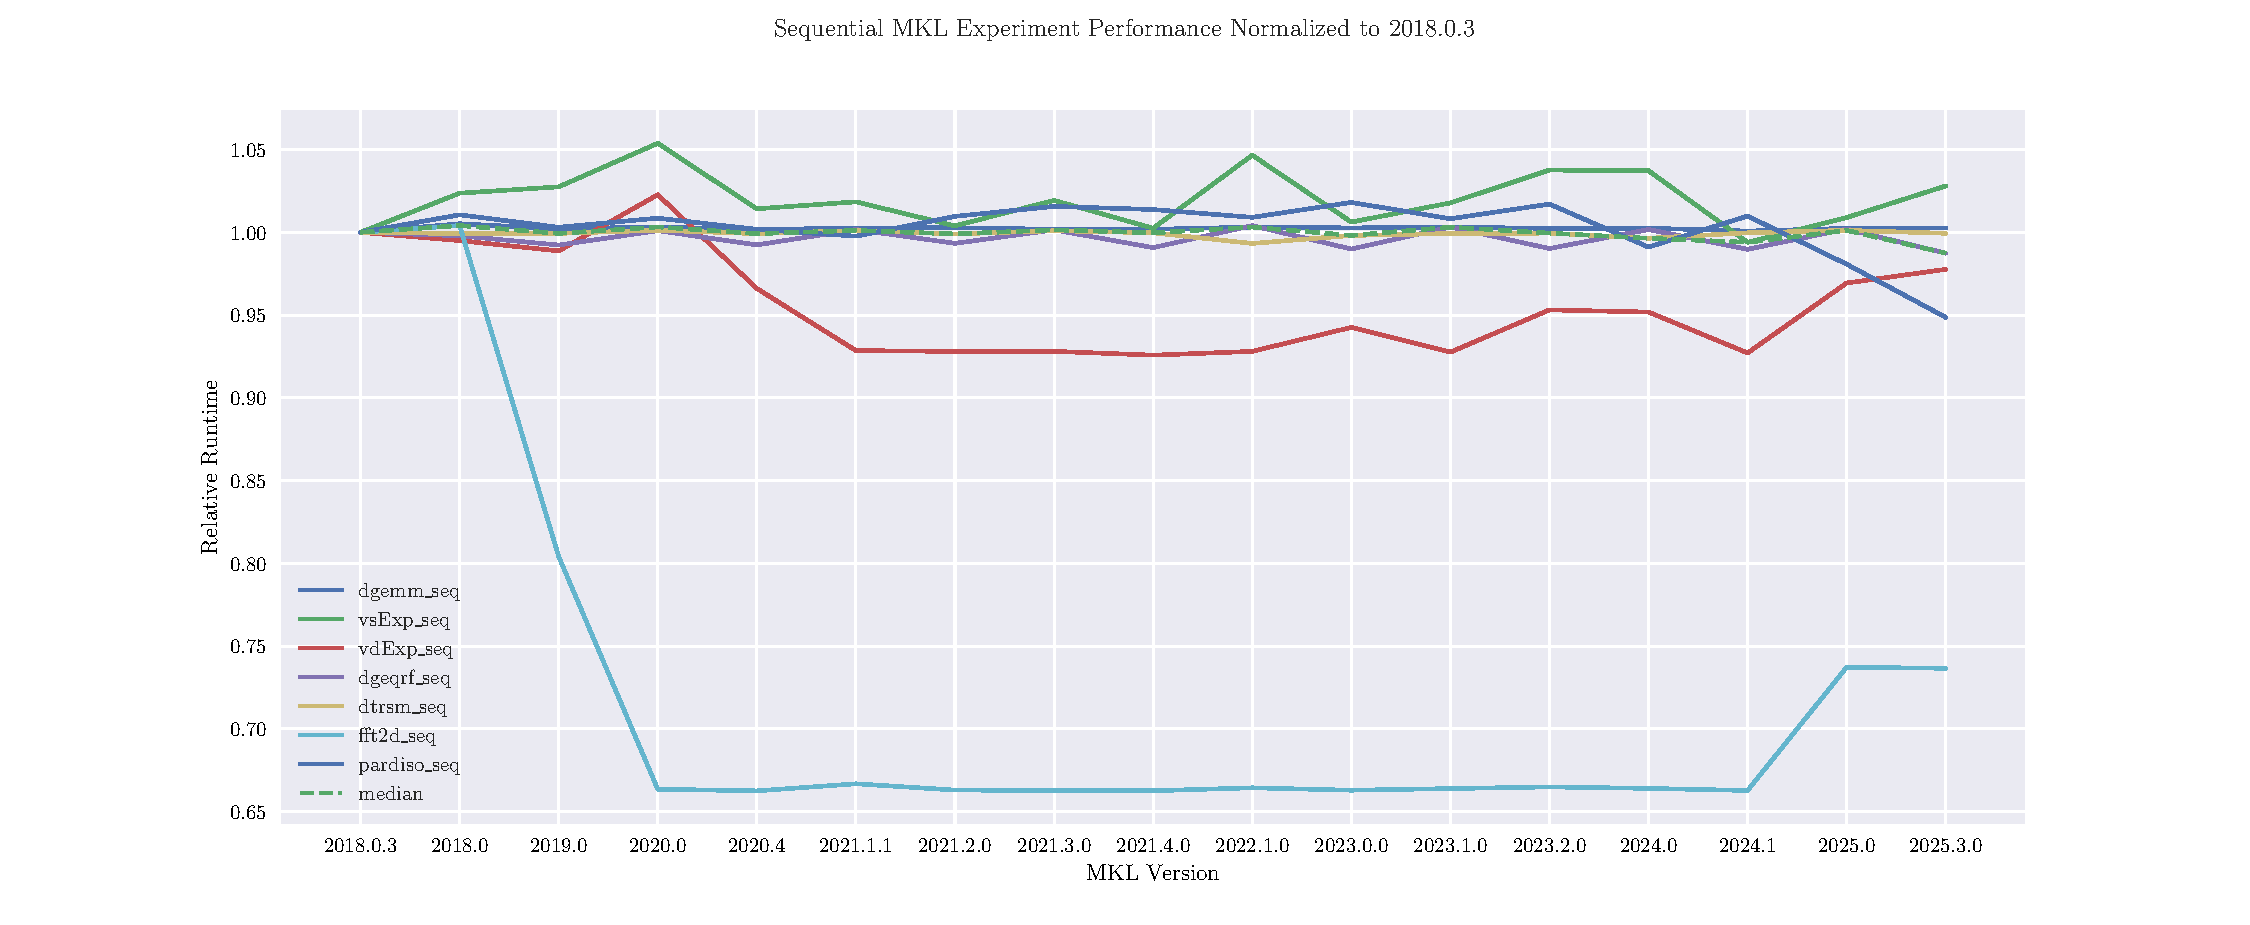
\includegraphics[width=12cm, page=1]{assets/seq_overview.pdf}
\end{center}
\end{frame}

